\chapter{Pasivní detektory používané k monitorování kosmického záření}\label{sec:detektory_detektory}
Pasivní detektory nepotřebují napájení, jsou dobře skladné (malé rozměry, malá hmotnost) a bezpečné, což je činí vhodnými měřícími prostředky ve vesmíru. Mezi jejich hlavní zápory patří, že nedodávají data v reálném čase a že pro vyhodnocení musí být dopraveny na Zem do příslušné laboratoře \cite{benton}.

K monitorování kosmického záření se používají detektory založené opticky stimulované luminiscenci (OSLD), termoluminiscenční detektory (TLD) a detektory stop v pevné fázi (TED, nuclear track etched detectors/solid state nuclear detectors). OSLD se využívají pouze okrajově a tato práce o nich nepojednává.

Výstupem z TLD je dávka, která se absorbovala v detektoru za celý čas měření. Oproti tomu pomocí TED je možné změřit $\mathit{LET}$ spektrum v rozsahu, který je rozebrán dále v textu; $\mathit{LET}$ je lineární přenos energie. Kombinací dat z TLD a z TED lze určit celkový dávkový ekvivalent \cite{benton}.
\section{Termoluminiscenční detektory}\label{sec:detektory_TLD}
Vyhodnocování TLD je založeno na jevu termoluminiscence: při zahřátí na teplotu, která je vlastní pro daný materiál a vyhodnocovací cyklus, se vyzáří světlo, jehož množství je přímo úměrné množství absorbované energie v detektoru. Důležitým pojmem je vyhřívací křivka TLD, což je závislost světelného toku (respektive elektrického signálu z fotonásobiče) na teplotě. Odezva TLD se určí právě z této křivky (např. jako plocha pod křivkou, plocha pod píkem, výška píku \cite{dosis}) a na základě kalibrační křivky lze dopočítat absorbovanou dávku. Kalibrační křivka se získává ozařováním TLD zdroji se známým dávkovým příkonem. Vzhledem k velké energetické a druhové rozmanitosti kosmického záření je třeba ozařovat dávkami v dostatečném rozsahu. 

TLD měří spolehlivě částice s $\mathit{LET}$ nižším než cca 10 keV/$\mu$m (tato hodnota se liší pro různé materiály), pro vyšší hodnoty $\mathit{LET}$ se účinnost TLD snižuje \cite{passDetectors}. Pro lepší popis tohoto jevu se zavádí veličina relativní odezva detektoru $\mathit{RR}$ (relative response)
\begin{equation}
  \mathit{RR}=\frac{\left(TL_{\text{odezva}}/D_{\text{tkáň}}\right)_Y}{\left(TL_{\text{odezva}}/D_{\text{tkáň}}\right)_{\gamma}},
  \label{eq:detektory_TLD_RR}
\end{equation}
kde $(TL_{\text{odezva}})_Y$, resp. $(TL_{\text{odezva}})_{\gamma}$ je odezva TLD po ozáření dávkou $(D_{\text{tkáň}})_Y$, resp. $(D_{\text{tkáň}})_{\gamma}$, přičemž tyto dávky jsou si číselně rovny. Jinak řečeno $\mathit{RR}$ je definována jako poměr odezev po ozáření stejnou dávkou v tkáni způsobenou částicemi $Y$ a referenčním zářením $\gamma$ \cite{TLD_RR}. 

Na vývoj $\RR$ se podíváme u dvou TLD používaných Oddělením dozimetrie záření ÚJF AV ČR (v dalším textu je používána anglická zkratka NPI). Jedná se o detektory Al$_2$O$_3$:C a CaSO$_4$:Dy, které se jmenují podle výrobních materiálů. Tyto detektory byly, resp. jsou používány v experimentech DOSIS a DOSIS3D. V tab. \ref{tab:detektory_TLD_RR} jsou hodnoty $\RR$ těchto detektorů pro částice s různým $\LET$ získané při experimentálním ozařování \cite{TLD_RR}. Lze pozorovat, že s rostoucím $\LET$ relativní odezva u obou detektorů klesá, u Al$_2$O$_3$:C mnohem rychleji než u CaSO$_4$:Dy; pro názornost jsou data z tabulky znázorněny i v grafu, viz \ref{fig:detektory_TLD_RR}. Pro zpřesnění měření je potřeba provést korekci TL odezev, více informací v
\cite{TLD_RR}.
\begin{table}[h]
  \centering
  \begin{tabular}{llll}
	\toprule
	Částice&$\LET$ [keV/$\mu$m]&Al$_2$O$_3$:C & CaSO$_4$:Dy\\
	\midrule
	He&$2,16$ &$0,77 \pm0,05$&$1,01\pm 0,09$\\
	O &$20,00$ &$0,47 \pm0,04$&$0,95\pm 0,06$\\
	Ar&$92,00$ &$0,32 \pm0,02$&$0,59\pm 0,04$\\
	Fe&$411,00 $ &$0,25 \pm0,02$&$0,44\pm 0,03$\\
\bottomrule
  \end{tabular}
  \caption{Relativní odezvy $\RR$ dvou TL detektorů používaných NPI pro částice s různým $\LET$. Data byla získána při experimentálním ozařování detektorů částicemi se známým $\LET$ \cite{TLD_RR}.}
  \label{tab:detektory_TLD_RR}
\end{table}
\begin{figure}[h]
  \centering
  % GNUPLOT: LaTeX picture with Postscript
\begingroup
  \makeatletter
  \providecommand\color[2][]{%
    \GenericError{(gnuplot) \space\space\space\@spaces}{%
      Package color not loaded in conjunction with
      terminal option `colourtext'%
    }{See the gnuplot documentation for explanation.%
    }{Either use 'blacktext' in gnuplot or load the package
      color.sty in LaTeX.}%
    \renewcommand\color[2][]{}%
  }%
  \providecommand\includegraphics[2][]{%
    \GenericError{(gnuplot) \space\space\space\@spaces}{%
      Package graphicx or graphics not loaded%
    }{See the gnuplot documentation for explanation.%
    }{The gnuplot epslatex terminal needs graphicx.sty or graphics.sty.}%
    \renewcommand\includegraphics[2][]{}%
  }%
  \providecommand\rotatebox[2]{#2}%
  \@ifundefined{ifGPcolor}{%
    \newif\ifGPcolor
    \GPcolortrue
  }{}%
  \@ifundefined{ifGPblacktext}{%
    \newif\ifGPblacktext
    \GPblacktexttrue
  }{}%
  % define a \g@addto@macro without @ in the name:
  \let\gplgaddtomacro\g@addto@macro
  % define empty templates for all commands taking text:
  \gdef\gplbacktext{}%
  \gdef\gplfronttext{}%
  \makeatother
  \ifGPblacktext
    % no textcolor at all
    \def\colorrgb#1{}%
    \def\colorgray#1{}%
  \else
    % gray or color?
    \ifGPcolor
      \def\colorrgb#1{\color[rgb]{#1}}%
      \def\colorgray#1{\color[gray]{#1}}%
      \expandafter\def\csname LTw\endcsname{\color{white}}%
      \expandafter\def\csname LTb\endcsname{\color{black}}%
      \expandafter\def\csname LTa\endcsname{\color{black}}%
      \expandafter\def\csname LT0\endcsname{\color[rgb]{1,0,0}}%
      \expandafter\def\csname LT1\endcsname{\color[rgb]{0,1,0}}%
      \expandafter\def\csname LT2\endcsname{\color[rgb]{0,0,1}}%
      \expandafter\def\csname LT3\endcsname{\color[rgb]{1,0,1}}%
      \expandafter\def\csname LT4\endcsname{\color[rgb]{0,1,1}}%
      \expandafter\def\csname LT5\endcsname{\color[rgb]{1,1,0}}%
      \expandafter\def\csname LT6\endcsname{\color[rgb]{0,0,0}}%
      \expandafter\def\csname LT7\endcsname{\color[rgb]{1,0.3,0}}%
      \expandafter\def\csname LT8\endcsname{\color[rgb]{0.5,0.5,0.5}}%
    \else
      % gray
      \def\colorrgb#1{\color{black}}%
      \def\colorgray#1{\color[gray]{#1}}%
      \expandafter\def\csname LTw\endcsname{\color{white}}%
      \expandafter\def\csname LTb\endcsname{\color{black}}%
      \expandafter\def\csname LTa\endcsname{\color{black}}%
      \expandafter\def\csname LT0\endcsname{\color{black}}%
      \expandafter\def\csname LT1\endcsname{\color{black}}%
      \expandafter\def\csname LT2\endcsname{\color{black}}%
      \expandafter\def\csname LT3\endcsname{\color{black}}%
      \expandafter\def\csname LT4\endcsname{\color{black}}%
      \expandafter\def\csname LT5\endcsname{\color{black}}%
      \expandafter\def\csname LT6\endcsname{\color{black}}%
      \expandafter\def\csname LT7\endcsname{\color{black}}%
      \expandafter\def\csname LT8\endcsname{\color{black}}%
    \fi
  \fi
    \setlength{\unitlength}{0.0500bp}%
    \ifx\gptboxheight\undefined%
      \newlength{\gptboxheight}%
      \newlength{\gptboxwidth}%
      \newsavebox{\gptboxtext}%
    \fi%
    \setlength{\fboxrule}{0.5pt}%
    \setlength{\fboxsep}{1pt}%
\begin{picture}(7936.00,5102.00)%
    \gplgaddtomacro\gplbacktext{%
      \csname LTb\endcsname%
      \put(814,704){\makebox(0,0)[r]{\strut{}0.2}}%
      \csname LTb\endcsname%
      \put(814,1163){\makebox(0,0)[r]{\strut{}0.3}}%
      \csname LTb\endcsname%
      \put(814,1622){\makebox(0,0)[r]{\strut{}0.4}}%
      \csname LTb\endcsname%
      \put(814,2082){\makebox(0,0)[r]{\strut{}0.5}}%
      \csname LTb\endcsname%
      \put(814,2541){\makebox(0,0)[r]{\strut{}0.6}}%
      \csname LTb\endcsname%
      \put(814,3000){\makebox(0,0)[r]{\strut{}0.7}}%
      \csname LTb\endcsname%
      \put(814,3459){\makebox(0,0)[r]{\strut{}0.8}}%
      \csname LTb\endcsname%
      \put(814,3919){\makebox(0,0)[r]{\strut{}0.9}}%
      \csname LTb\endcsname%
      \put(814,4378){\makebox(0,0)[r]{\strut{}1.0}}%
      \csname LTb\endcsname%
      \put(814,4837){\makebox(0,0)[r]{\strut{}1.1}}%
      \csname LTb\endcsname%
      \put(946,484){\makebox(0,0){\strut{}$1$}}%
      \csname LTb\endcsname%
      \put(3144,484){\makebox(0,0){\strut{}$10$}}%
      \csname LTb\endcsname%
      \put(5341,484){\makebox(0,0){\strut{}$100$}}%
      \csname LTb\endcsname%
      \put(7539,484){\makebox(0,0){\strut{}$1000$}}%
    }%
    \gplgaddtomacro\gplfronttext{%
      \csname LTb\endcsname%
      \put(176,2770){\rotatebox{-270}{\makebox(0,0){\strut{}$\mathit{RR}$ [-]}}}%
      \put(4242,154){\makebox(0,0){\strut{}$\mathit{LET}$ [keV/$\mu$m]}}%
      \csname LTb\endcsname%
      \put(6552,4538){\makebox(0,0)[r]{\strut{}Al$_2$O$_3$:C}}%
      \csname LTb\endcsname%
      \put(6552,4066){\makebox(0,0)[r]{\strut{}CaSO$_4$:Dy}}%
    }%
    \gplbacktext
    \put(0,0){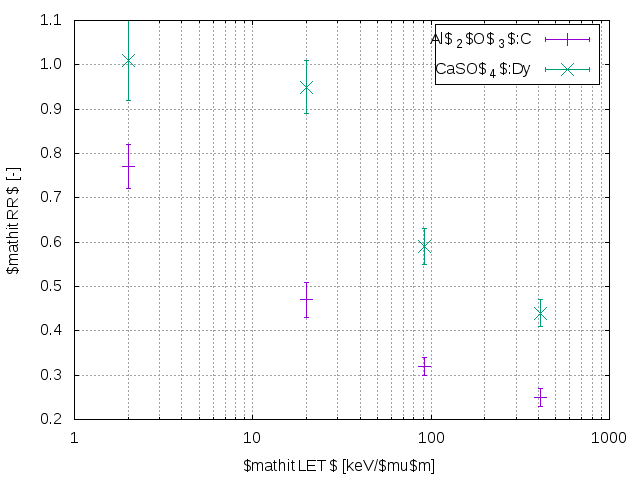
\includegraphics{TLD_RR}}%
    \gplfronttext
  \end{picture}%
\endgroup

  \caption{Data z tab. \ref{tab:detektory_TLD_RR} vynesená do grafu, tj. relativní odezva dvou detektorů používaných NPI pro částice s různým $\LET$.}
  \label{fig:detektory_TLD_RR}
\end{figure}
%možnost dát obrázek, avšak moc to nejde (z gnuplotu), zkusit https://tex.stackexchange.com/questions/135308/how-can-we-import-the-gnuplot-output-in-latex
\section{Detektory stop v pevné fázi}

\begin{equation}
  V=\frac{\sqrt{\left( 1-B^2 \right)^2}+4A^2}{1-B^2},
  \label{eq:pomerLepRychlosti}
\end{equation}
kde
\begin{align*}
  A&=\frac{a}{2V_Bt},\\
  B&=\frac{b}{2V_Bt}
\end{align*}

\begin{equation}
  k_{\theta}=\frac{V^2}{V^2-1}
  \label{}
\end{equation}



%vyhodnocování OSLD probíhá pomocí referenčního zdroje (ten vztah asi nepsat) (dosis, s. 7); OSLD detektory se tato práce nezabývá, takže spíš ne

%napsat z ceho jsou vyrobene (nebo spis co presne jsou) TLD pouzivane NPI (prasek, krystal atd.)

%HSP1000 -> jediny v Evrope!!!!!!!!!!! (viz stranky ODZ UJF AVCR) -> to uz je v praktickaCast


%Nevýhodou pasivních detektorů je skutečnost, že po každém měření musely být dopraveny zpět na Zem do příslušné laboratoře a teprve tam byly vyhodnoceny; avšak oproti aktivním detektorům nemusejí být napájeny proudem, což je v prostředí ISS velmi praktické. %toto asi až to další kapitoly o detektorech

